%----------------------------------------------------------------------------------------
%	Inställningar och dokumentkonfiguration
%----------------------------------------------------------------------------------------

\documentclass[a4paper,11pt]{report} % A4-sida och 11 punkters fontstorlek

\usepackage[T1]{fontenc} % 8-bitarskodning som har 256 glyfer
\usepackage[swedish]{babel} % Svenskt språk
\usepackage[utf8]{inputenc} % För svenska tecken
\usepackage{dtklogos} % Logos
\usepackage{wallpaper} % Bakgrundsbild

\usepackage{fancyhdr} % Specialsidhuvud och sidfot
\pagestyle{fancyplain} % Använd sidhuvud och sidfot på alla sidor
\fancyhead[L]{Laborationsrapport -- Kursnamn XDVXXX} % Titel till vänster i sidhuvud
\fancyhead[C]{} % Tomt i mitten
\fancyhead[R]{} % Tomt till höger
\fancyfoot[L]{} % Tomt till vänster
\fancyfoot[C]{} % Tomt i mitten
\fancyfoot[R]{\thepage} % Sidnumrering till höger i sidfoten
\renewcommand\thesection{\arabic{section}} % Section beter sig som i dokumentklassen article

%----------------------------------------------------------------------------------------
%	Titelsektion
%----------------------------------------------------------------------------------------
\newcommand\BackgroundPic{
    \put(0,-100){
    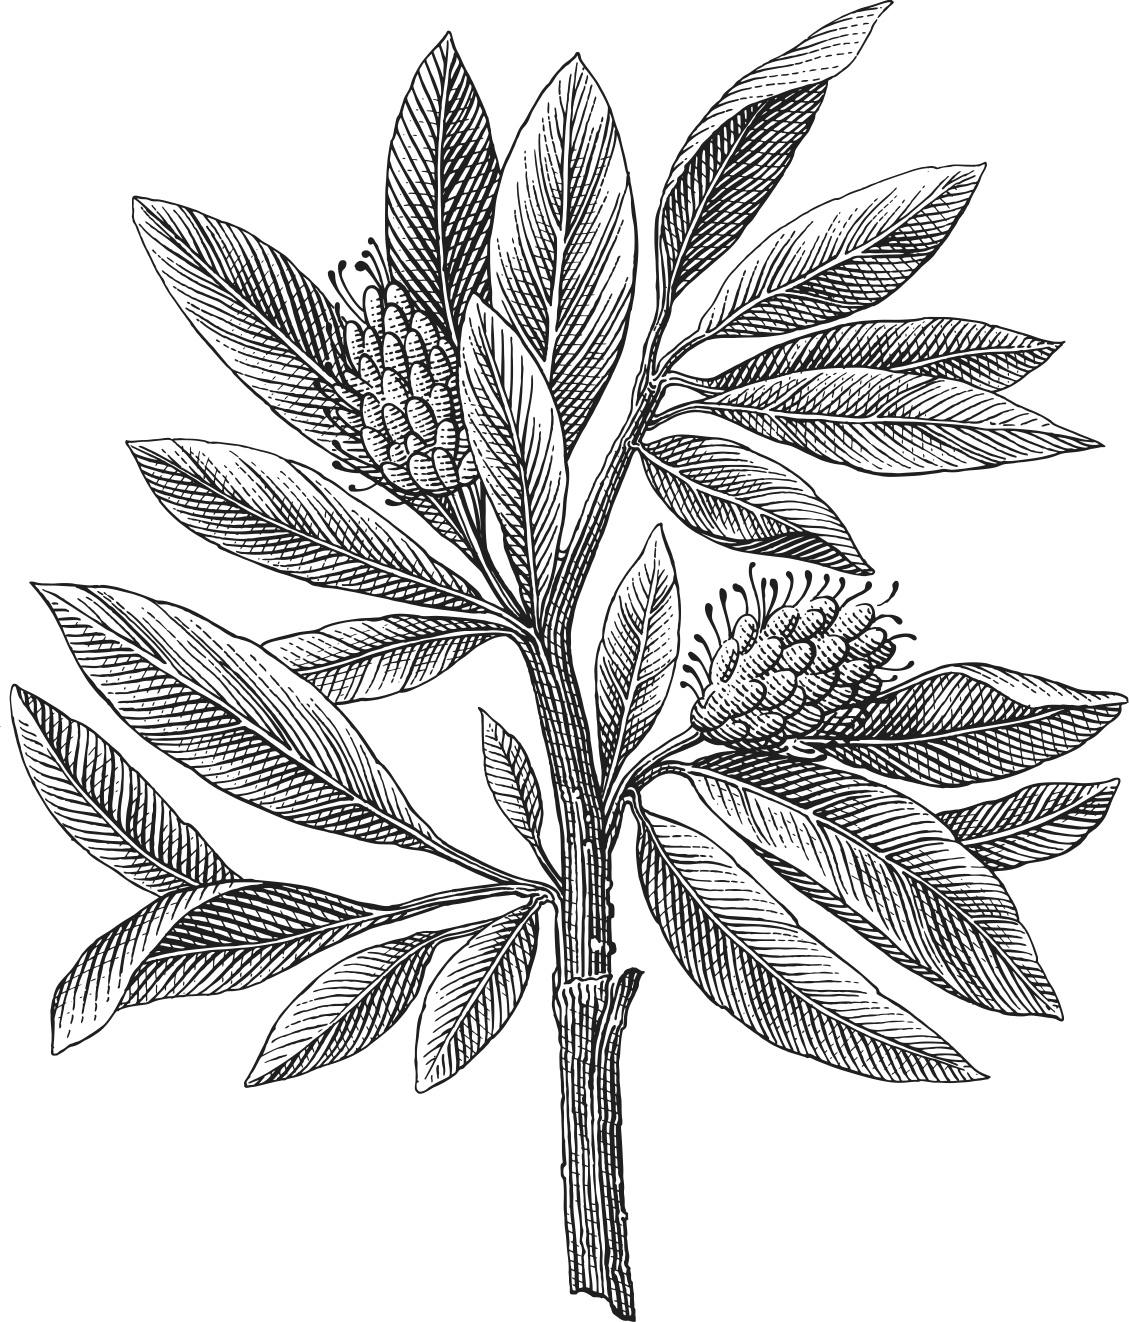
\includegraphics[keepaspectratio,scale=0.65]{img/lnu_etch.png} % Bakgrundsbild
    }
}
\newcommand\BackgroundPicLogo{
    \put(15,700){
    
\includegraphics[keepaspectratio,scale=0.10]{img/logo.png} % Logga i vänstra hörnet
    }
}

\newcommand{\horrule}[1]{\rule{\linewidth}{#1}} % Skapa hortisontell linje

\title{	\vspace{-10cm}
    \normalfont \normalsize
    \textsc{Linnéuniversitetet} \\ [25pt] % Universitetes namn
    Laborationsrapport -- Kursnamn XDVXXX % Typ och kurs
    \horrule{0.5pt} \\[0.4cm] % Tunn linje högst upp
    \huge Laborationens titel -- Ändra mig \\ % Arbetes titel
    \horrule{0.5pt} \\[0.4cm] % Tunn linje längst ner
}

\author{Studentnamn1, Studentnamn2, Studentnamn3} % Författarnas namn

\date{\normalsize\today} % Dagens datum

\begin{document}
\AddToShipoutPicture*{\BackgroundPic} % Lägger in backgrundsbild på första sidan
\AddToShipoutPicture*{\BackgroundPicLogo}
\maketitle % Skriv ut titeln
\abstract{Lorem ipsum dolor sit amet, consectetur adipiscing elit. Mauris eget magna vel lacus laoreet lobortis sed a ligula. Phasellus dolor ligula, molestie eget vestibulum sed, tempor nec orci. Pellentesque quis quam faucibus, iaculis purus sit amet, vehicula nibh. Suspendisse potenti. In hac habitasse platea dictumst. Curabitur dictum adipiscing massa, ac semper magna pretium pharetra. Ut sem massa, pellentesque et tincidunt a, suscipit id nunc. Vivamus tristique arcu non eros sagittis tincidunt. Proin hendrerit, elit eu facilisis dignissim, purus erat consequat eros, a condimentum tellus magna et ligula. Proin vitae magna porta enim porttitor pellentesque sed ac nisi. Cras elementum sollicitudin tincidunt. Sed varius tellus a dui rutrum egestas. Morbi tincidunt pretium libero, non molestie turpis porttitor ut.} % Här skrivs sammanfattningen
\newpage
\noindent % Tabba inte in på första meningen
Detta dokument använder \LaTeX. För innehållsbeskrivning och längd på varje stycke, se projektbeskrivningen.

%------------------------------------------------
%	Introduktion
%
%   Här skriver du om laborationen i allmänhet,
%   de tekniker, programvaror och liknande du
%   använt under labben
%------------------------------------------------
\section{Introduktion}
Curabitur pellentesque, nulla et semper pharetra, neque sem tincidunt ipsum, nec sodales odio purus gravida tellus. Nulla euismod molestie nisi, pretium bibendum neque iaculis nec.
\subsection{Laborationsmiljö}
Laborationsmiljön bestod av...
\subsection{VMware Workstation}
Beskrivning av programvaran.
\subsection{Apache Web Server}
Beskrivning av programvaran.
%------------------------------------------------
%	Genomförande
%   Denna delen innehåller de praktiska saker du
%   gjort under laborationen. Du skriver även
%   om utfallet av labben och de resultat du fick
%   när du arbetade med laborationen.
%------------------------------------------------
\section{Genomförande och resultat}
Vivamus a tortor non augue congue euismod. Duis venenatis mi sed porta pellentesque. Aliquam feugiat quam nec condimentum laoreet. Fusce lobortis, nisl at congue sodales, nulla sem pellentesque erat, eu adipiscing est eros nec dolor. Nulla dictum cursus erat, nec hendrerit elit interdum ut. Donec ornare justo nulla, rutrum pretium leo fermentum a. Sed lacinia nulla sit amet porttitor imperdiet.
%------------------------------------------------
%	Slutsatser och reflektion
%------------------------------------------------
\section{Slutsatser och reflektion}
Cras nulla leo, aliquet eget elementum nec, luctus in justo. Fusce fermentum leo et elementum pellentesque. Sed lobortis a lectus sit amet ultrices. Nulla sodales enim eu eros fermentum, vitae sollicitudin lectus aliquet. Quisque tristique purus urna. Pellentesque porttitor, ligula ut facilisis commodo, orci tellus eleifend sem, eget tempus mauris dui sit amet nunc. Nullam id mauris nisl. Phasellus scelerisque nulla faucibus risus tincidunt interdum. Donec eu urna diam. Pellentesque aliquet euismod ipsum, dictum pretium odio rhoncus et.
\newpage
%------------------------------------------------
%	Litteraturlista
%------------------------------------------------
Använd IEEEs system för referenser, för att underlätta referenshanteringen rekommenderar jag \BibTeX. Här citerar jag small \cite{small} och här citerar jag big \cite{big} och här är exempel på en elektronisk källa \cite{sven02}. Se \emph{referenser.bib} för formatering av litteraturlista i \BibTeX-format. Denna text ska \emph{inte} finnas med i den slutgiltiga rapporten.
\bibliographystyle{IEEEtran}
\bibliography{referenser}
\end{document}
